\documentclass[a4paper,12pt]{article}


\usepackage[utf8]{inputenc}
\usepackage[T1]{fontenc}
\usepackage[polish]{babel}
\usepackage{color}
\usepackage{xcolor}
\usepackage{geometry}
\usepackage{fontspec}
\usepackage{geometry}
\usepackage{subfig}
\geometry{left=2.5cm,right=2.5cm,top=2.5cm,bottom=2.5cm}
\usepackage{multicol}
\usepackage{fancyhdr}
\linespread{1.5}
\colorlet{shadecolor}{gray!40}
\usepackage{listings}
\usepackage{pdfpages}
\lstdefinestyle{mystyle}{
	%backgroundcolor=\color{shadecolor}
	commentstyle=\footnotesize\color{blue},
	keywordstyle=\color{red},
	numberstyle=\footnotesize\color{black},
	stringstyle=\color{black},
	basicstyle=\footnotesize,
	breakatwhitespace=false,
	breaklines=true, captionpos=b,
	keepspaces=true, numbers=left,
	numbersep=5pt, showspaces=false,
	showstringspaces=false, showtabs=false,
	tabsize=2,	
}
\lstset{style=mystyle}
\setlength{\parindent}{1.25cm}


\usepackage{amsmath}
\usepackage{graphicx}
\usepackage{hyperref}
\usepackage{fancyhdr}
\usepackage{tocloft}

\newtheorem{theorem}{Twierdzenie}

\title{Numeryczne wyznaczanie rozwiązań równania Burgersa przy pomocy metody różnic skończonych}
\author{Konrad Bonicki, Tomasz Orzechowski, Maciej Pestka}
\date{\today}

\begin{document}

\maketitle

\tableofcontents
\newpage

\section{Wprowadzenie}
W tej pracy przybliżymy równanie Burgersa oraz jego zastosowania, jego rozwiązanie analityczne i metody, które użyliśmy podczas pisania programu, który numerycznie wyznacza rozwiązania przytoczonego równania.

\section{Równanie Burgersa}
Równanie Burgersa w ogólnej postaci jest fundamentalnym, nieliniowym, parabolicznym równaniem różniczkowym cząstkowym drugiego rzędu występującym w przeróżnych obszarach zastosowań matematyki, takich jak mechanika płynów, dynamika gazów oraz płynność ruchu:
\begin{equation}
\frac{\partial u}{\partial t} + u \frac{\partial u}{\partial x} = v \frac{\partial ^2 u}{\partial x^2}
\end{equation}
gdzie: 
\begin{itemize}
\item $t$ - zmienna niezależna zwykle interpretowana jako czas,
\item $x$ - zmienna niezależna zwykle interpretowana jako położenie,
\item $u(x,t)$ - zmienna zależna zwykle interpretowana jako prędkość płynu,
\item $v$ - stały parametr, zwykle interpretowany jako lepkość płynu.
\end{itemize}

\section{Transformacja Hopf-Cole'a}
Transformacja Cole-Hopf’a jest zmianą zmiennych, która umożliwia przekształcenie specjalnego rodzaju parabolicznych równań różniczkowych cząstkowych z nieliniowością kwadratową w liniowe równanie cieplne. Wygląda następująco:
\begin{equation}
u(x,t)=-2v\frac{\theta _x (x,t)}{\theta (x,t)}
\end{equation}
$$u=-2v\frac{\theta _x}{\theta}$$
Liczymy pochodne cząstkowe z (2), aby podstawić je potem do równania Burgersa
	$$u_x=-2v\frac{\theta _{xx} \theta - \theta ^{2}_{x}}{\theta ^2}, \quad u_t=-2v\frac{\theta _{xt}\theta - \theta _x \theta _t}{\theta ^2}$$
	$$u_{xx}=-2v\frac{\theta _{xxx}\theta ^2 - 3\theta \theta _x \theta _{xx} + 2\theta ^{3}_{x}}{\theta ^3}$$
	Podstawiamy teraz to co nam wyszło do równania Burgersa:
	$$u_t + u u_x = v u_{xx}$$
$$-2v \frac{\theta _{xt}\theta - \theta _x \theta _t }{\theta ^2} + 4 v^2 \frac{\theta \theta _x \theta _{xx} - \theta ^{3}_{x}}{\theta ^3} = -2v^2\frac{\theta _{xxx} \theta ^2 - 3\theta \theta _x \theta _{xx} + 2\theta ^{3}_{x}}{\theta ^3}$$
$$-2v\theta (\theta _{xt} \theta - \theta _x \theta _t ) +4v^2 (\theta \theta _x \theta _{xx} - \theta ^{3}_{x}) = -2v^2(\theta _{xxx} \theta ^2 - 3\theta \theta _x \theta _{xx} + 2\theta ^{3}_{x})$$
$$\theta ^2 \theta _{xt} - \theta \theta _x \theta _t -2v \theta \theta _x \theta _{xx} +2\theta^{3}_{x}=v \theta _{xxx} \theta ^2 -3v\theta \theta _x \theta _{xx} +2 \theta ^{3}_{x}$$
$$\theta \theta _{xt} - \theta _x \theta _t -2v\theta _x \theta _{xx}= v\theta \theta _{xxx} - 3v\theta _x \theta _{xx}$$
$$\theta \theta _{xt} - \theta _x \theta _t = v(\theta \theta _{xxx} - \theta _x \theta _{xx})$$
$$\theta \frac{\partial 
\theta ^2}{\partial x \partial t}- \frac{\partial \theta}{\partial x} \frac{\partial \theta}{\partial t} = v(\theta \frac{\partial ^3 \theta}{\partial x^3}-\frac{\partial \theta}{\partial x}\frac{\partial ^2 \theta}{\partial x^2})$$
$$\frac{\partial \theta}{\partial t}(\theta \frac{\partial \theta}{\partial x}-\frac{\partial \theta}{\partial x})=v\frac{\partial ^2 \theta}{\partial x^2}(\theta \frac{\partial \theta}{\partial x}-\frac{\partial \theta}{\partial x})$$
$$\theta \theta _x - \theta _x \neq 0$$
$$ \theta _t = v \theta _{xx}$$
Po podstawieniu transformacji Hopf-Cole'a do równania Burgersa otrzymaliśmy równanie ciepła.

\section{Rozwiązanie analityczne przy pomocy transformacji Hopf-Cole'a}
Równanie Burgersa: $$u_t +uu_x=vu_{xx}$$
Warunek początkowy: $$u(x,0)=\sin (\pi x), \quad 0<x<1,$$ Warunki brzegowe: $$u(0,t)=u(1,t)=0, \quad t>0. $$ Transformacja Hopf-Cole'a: $$u(x,t)=-2v\frac{\theta _x (x,t)}{\theta (x,t)}$$ Z równania Burgersa z poprzedniego punktu mamy: $$ \theta _t = v \theta _{xx}, \quad 0<x<1 \quad t>0$$
Warunek początkowy $\theta :$
$$u(x,0)=-2v\frac{\theta _x (x,0)}{\theta (x,0)}, \quad \theta (x,0) \neq 0$$
$$\sin (\pi x) = -2v\frac{\theta _x (x,0)}{\theta (x,0)}$$
$$-\frac{1}{2v}\sin (\pi x)=\frac{\theta _x (x,0)}{\theta (x,0)}$$
$$-\frac{1}{2v} \int^x_0 \sin (\pi x)dx = \int^x_0 \frac{\theta _x (x,0)}{\theta (x,0)}dx $$
$$-\frac{1}{2v} [-\frac{1}{\pi}\cos (\pi x)]^{x=x}_0=[ln[\theta (x,0)]]^{x=x}_0$$
$$\frac{1}{2v\pi}(\cos (\pi x)-1)=ln[\theta (x,0)]-ln[\theta (0,0)]$$
Wyznaczamy $\theta (0,0)$:
$$u(0,0)=-2v\frac{\theta _x (0,0)}{\theta (0,0)}$$
$$u(0,0)=\sin (\pi 0)=0$$
$$0=\frac{\theta _x (0,0)}{\theta (0,0)}$$
$$\int^x_0 0 dx = \int^x_0 \frac{\theta _x (0,0)}{\theta (0,0)} dx$$
$$ln(\theta(0,0))=0$$
$$\theta (0,0) = e^0=1$$
Co daje:
$$\theta (x,0)= e^{\frac{1}{2v\pi}(\cos (\pi x)-1)}, \quad 0<x<1$$
Warunki brzegowe $\theta:$
$$u(0,t)=u(1,t)=0$$
$$-2v\frac{\theta _x (0,t)}{\theta (0,t)}=-2v\frac{\theta _x (1,t)}{\theta (1,t)}=0,\quad \theta (0,t)\neq 0 \quad \theta (1,t) \neq 0$$
$$\theta _x (0,t) = \theta _x (1,t) =0, \quad t>0$$
Rozwiązanie: $$\theta _t = v \theta _{xx}, \quad 0<x<1 \quad t>0$$
Do rozwiązania tego równania wykorzystam metodę Fouriera:
$$\theta (x,t)=X(x)T(t)$$
$$X(x)T`(t)=vX``(x)T(t)$$
$$\frac{T`(t)}{vT(t)}=\frac{X``(x)}{X(x)}=-\lambda ^2$$
$$T`(t)=-\lambda ^2 vT(t)$$
$$T(t)=e^{-\lambda ^2 vt}$$
$$X``(x)=-\lambda ^2X(x)$$
$$X(x)=A\sin(\lambda x)+B\cos(\lambda x)$$
$$\theta (x,t) = (A\sin(\lambda x)+B\cos(\lambda x))e^{-\lambda ^2 vt}$$
$$\theta _x (x,t)=(A\cos(\lambda x)-B\sin(\lambda x))e^{-\lambda ^2 vt}$$
$$\theta _x (0,t)=0$$
$$(A\cos(\lambda 0)-B\sin(\lambda 0))e^{-\lambda ^2 vt}=0$$
$$Ae^{-\lambda ^2 vt}=0 <=> A =0$$
$$\theta _x (1,t)=0$$
$$(-B\sin(\lambda))e^{-\lambda ^2 vt}=0$$
Funkcja sinus przyjmuje wartości 0 dla $\lambda=n\pi,\quad n=0,1,2,...$, omijamy rozwiązanie trywialne $B=0$:
\\
\\
Wracamy z wyznaczonymi współczynnikami do momentu przed różniczkowaniem funkcji $\theta$:
$$\theta  (x,t) =B_0+ \sum_{n=1}^\infty B_n \cos (n\pi x) e^{-n^2 \pi ^2 vt}$$
Wyznaczamy współczynniki $B_n\quad (n=0,1,2,...)$:
$$B_0 = \int_0^1 e^{\frac{1}{2v\pi}(\cos (\pi x)-1)}dx 
=e^{-\frac{1}{2v\pi}}\int_0^1 e^{\frac{\cos (\pi x)}{2v\pi}}dx$$
$$B_n = 2\int_0^1 e^{\frac{1}{2v\pi}(\cos (\pi x)-1)}\cos (n \pi x)dx=2e^{-\frac{1}{2v\pi}}\int_0^1 e^{\frac{\cos (\pi x)}{2v\pi}}\cos (n \pi x)dx$$
Rozwiązanie:
$$u (x,t) = 2v\pi \frac{\sum_{n=1}^\infty B_n \sin (n\pi x) e^{-n^2 \pi ^2 vt}}{B_0+ \sum_{n=1}^\infty B_n \cos (n\pi x) e^{-n^2 \pi ^2 vt}}$$


\section{Metody numeryczne - wstęp}
Metod numerycznych używamy do rozwiązywania problemów matematycznych za pomocą operacji na liczbach. Metody numeryczne są wykorzystywane, gdy problem nie posiada rozwiązania analitycznego lub gdy takie rozwiązanie jest zbyt skomplikowane do zastosowania. W naszym projekcie korzystamy z metody różnic skończonych, metody Rungego-Kuty'ego oraz metody Eulera.

\section{Wzór Taylora}
Wzór Taylora jest ważnym narzędziem w analizie numerycznej:
\begin{theorem}
Jeśli $f \in C^n [a,b]$ i jeśli $f^{(n+1)}$ istnieje w przedziale otwartym $(a,b)$, to dla dowolnych punktów $c$ i $x$ z przedziału domkniętego $[a,b]$ mamy:
\begin{equation}
f(x)=\sum_{k=0}^n \frac{1}{k!}f^{(k)}(c)(x-c)^k + E_n (x),
\end{equation}
gdzie dla pewnego punktu $\xi$ leżącego między $c$ i $x$:
\begin{equation}
E_n (x) = \frac{1}{(n+1)!}f^{(n+1)}(\xi)(x-c)^{n+1}.
\end{equation}
\end{theorem}

\section{Metoda różnic skończonych}
Metoda różnic skończonych polega na przybliżaniu pochodnych za pomocą różnic skończonych. Zarówno dziedzina przestrzenna, jak i czasowa są dyskretyzowane, czyli dzielone na skończoną liczbę przedziałów, a wartości rozwiązania na końcach tych przedziałów są przybliżane przez rozwiązywanie równań algebraicznych zawierających różnice skończone i wartości z pobliskich punktów.

Wyznaczanie ilorazów różnicowych przy pomocy wzoru Taylora:

\begin{align*}
    u(x+h) &= u(x) + u'(x) \frac{(h)}{1!} + u''(x) \frac{(h-x)}{2!} + O(h^2) \\
    u(x) &= u(x) \\
    u(x-h) &= u(x) - u'(x) \frac{(h)}{1!} + u''(x) \frac{(-h-x)}{2!} + O(h^2)
\end{align*}

Przybliżenie pierwszej pochodnej:

\begin{align*}
    u'(x) &= Au(x+h) + Bu(x) + Cu(x-h) \\
    &= A(u(x) + hu'(x) + \frac{1}{2} u''(x)h^2) + B u(x) + C(u(x) - hu'(x) + \frac{1}{2} u''(x)h^2)
\end{align*}

\begin{align*}
    u(x) &: \quad A + B + C = 0 \\
    u'(x) &: \quad A h - Ch = 1 \\
    u''(x) &: \quad \frac{1}{2} h^2 A + \frac{1}{2} h^2 C = 0
\end{align*}

\begin{align*}
    A = \frac{1}{2h}, \quad B = 0, \quad C = -\frac{1}{2h}
\end{align*}

\begin{align*}
    u'(x) \approx \frac{1}{2h} u(x+h) + 0u(x) - \frac{1}{2h} u(x-h) = \frac{u(x+h) - u(x-h)}{2h}
\end{align*}

Przybliżenie drugiej pochodnej:

\begin{align*}
    u''(x) = A u(x+h) + B u(x) + C u(x-h)
\end{align*}

\begin{align*}
    u(x) &: \quad A + B + C = 0 \\
    u'(x) &: \quad A h - Ch = 0 \\
    u''(x) &: \quad \frac{1}{2} h^2 A + \frac{1}{2} h^2 C = 1
\end{align*}

\begin{align*}
    A = \frac{1}{h^2}, \quad B = -\frac{2}{h^2}, \quad C = \frac{1}{h^2}
\end{align*}

\begin{align*}
    u''(x) \approx \frac{1}{h^2} u(x+h) - \frac{2}{h^2} u(x) + \frac{1}{h^2} u(x-h) = \frac{u(x+h) - 2u(x) + u(x-h)}{h^2}
\end{align*}

\section{Metoda Eulera}
Metoda Eulera jest najprostszą metodą rozwiązywania równań różniczkowych zwyczajnych, opartą na wzorze Taylora. Opisuje ją wzór:
\begin{equation}
x(t+h) \approx x(t) + hf(t,x)
\end{equation}
Jej zaletą jest to, że nie trzeba różniczkować funkcji $f$, natomiast wadą jest konieczność wyboru bardzo małego kroku $h$.

\section{Metoda Rungego-Kutty}
Rozważmy ogólne równanie różniczkowe zwyczajne pierwszego rzędu:
\begin{equation}
    y' = f(t, y)
\end{equation}
z warunkiem początkowym \( y(t_0) = y_0 \).

\subsection*{Algorytm}
Metoda Rungego-Kutty drugiego stopnia jest jedną z metod numerycznych stosowanych do rozwiązywania równań różniczkowych zwyczajnych (ODE). Jest to rozwinięcie metody Eulera, które zwiększa dokładność przez uwzględnienie dodatkowych informacji o nachyleniu funkcji.
\begin{enumerate}
    \item \textbf{Krok początkowy:} 
    \begin{equation}
        y_0 = y(t_0)
    \end{equation}

    \item \textbf{Obliczenie przyrostów:}
    \begin{equation}
        k_1 = h f(t_n, y_n)
    \end{equation}
    \begin{equation}
        k_2 = h f\left(t_n + \frac{h}{2}, y_n + \frac{k_1}{2}\right)
    \end{equation}

    \item \textbf{Obliczenie następnej wartości \( y \):}
    \begin{equation}
        y_{n+1} = y_n + k_2
    \end{equation}

    \item \textbf{Aktualizacja czasu:}
    \begin{equation}
        t_{n+1} = t_n + h
    \end{equation}
\end{enumerate}
\section{Rozwiązanie równania Burgersa}
Rozważamy cztery równania różniczkowe cząstkowe.\\

Równanie transportu
\begin{equation}
\frac{\partial u}{\partial t}+\frac{\partial u}{\partial x}=0, 0\le x\le10, t>0
\end{equation}
\vspace{0.5cm}

Nielepkie równanie Burgersa
\begin{equation}
\frac{\partial u}{\partial t}+u\frac{\partial u}{\partial x}=0, 0\le x\le10, t>0
\end{equation}
\vspace{0.5cm}

Równanie ciepła
\begin{equation}
\frac{\partial u}{\partial t}-\beta\frac{\partial^{2} u}{\partial x^{2}}=0, 0\le x\le10, t>0, \beta>0
\end{equation}
\vspace{0.5cm}

Równanie Burgersa (nieliniowe, paraboliczne)
\begin{equation}
\frac{\partial u}{\partial t}+u\frac{\partial u}{\partial x}-\beta\frac{\partial^{2} u}{\partial x^{2}}=0, 0\le x\le10, t>0, \beta>0
\end{equation}
gdzie zmienne i parametry zostały opisane w rozdziale 2, pod równaniem (1).\\
Dla przypomnienia, $\beta$ jest współczynnikiem lepkości.
\vspace{0.5cm}

Naszym celem jest wykorzystanie metod różnic skończonych w celu znalezienia przybliżonych\\
wartości $u(x,t)$ rozwiązania wszystkich równań.\\
Najpierw określmy krok przestrzenny $h$ oraz krok czasowy $k$. Niech
\begin{equation}
\begin{split}
& u_{i,j}=u(x_{i},t_{j})=u(i\cdot h,j\cdot k),\\
& h=0.1, k=0.005, i\in[0,M-1], j\in[0,N-1], M,N\in\mathbb{N}
\end{split}
\end{equation}

Wtedy niech warunek początkowy wszystkich równań (funkcja Gaussa)
\begin{equation}
u_{i,0}=e^{-(x_{i}-x_{mid})^{2}}, x_{mid}=\frac{(M - 1) \cdot h}{2}=5
\end{equation}

Oraz niech warunki brzegowe wszystkich równań
\begin{equation}
u_{0,j}=u_{M-1,j}=0
\end{equation}

Niech 
\begin{equation}
\beta<\frac{h^{2}}{2k}\land\beta=0.99
\end{equation}
w celu uzyskania stabilności rozwiązań.
\newpage

Wtedy stosując metodę Eulera:\\
dla równania transportu
\begin{equation}
\begin{split}
& \frac{1}{k}(u_{i,j+1}-u_{i,j})+\frac{1}{2h}(u_{i+1,j}-u_{i-1,j})=0\\
& u_{i,j+1}=u_{i,j}-\frac{k}{2h}(u_{i+1,j}-u_{i-1,j})
\end{split}
\end{equation}
\begin{figure}[h]
\caption{Równanie transportu, metoda Eulera}
\centering
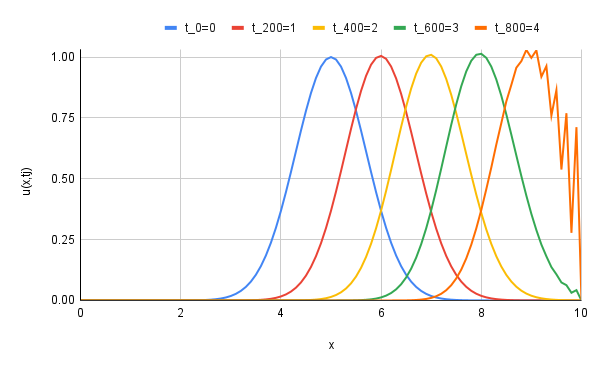
\includegraphics[width=0.85\textwidth]{rys/0.png}
\end{figure}
dla nielepkiego równania Burgersa
\begin{equation}
\begin{split}
& \frac{1}{k}(u_{i,j+1}-u_{i,j})+\frac{1}{4h}(u_{i+1,j}^{2}-u_{i-1,j}^{2})=0\\
& u_{i,j+1}=u_{i,j}-\frac{k}{4h}(u_{i+1,j}^{2}-u_{i-1,j}^{2})
\end{split}
\end{equation}
\begin{figure}[h]
\caption{Nielepkie równanie Burgersa, metoda Eulera}
\centering
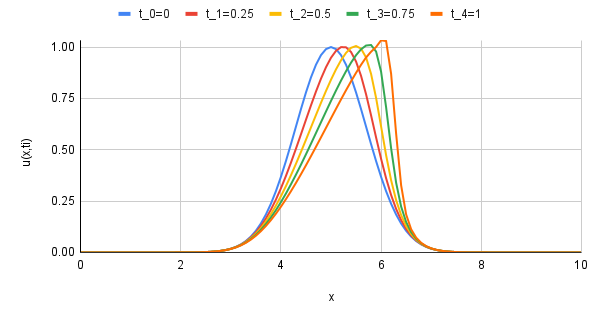
\includegraphics[width=0.85\textwidth]{rys/1.png}
\end{figure}
\newpage

dla równania ciepła
\begin{equation}
\begin{split}
& \frac{1}{k}(u_{i,j+1}-u_{i,j})-\frac{\beta}{h^{2}}(u_{i+1,j}-2u_{i,j}+u_{i-1,j})=0\\
& u_{i,j+1}=u_{i,j}+\frac{\beta k}{h^{2}}(u_{i+1,j}-2u_{i,j}+u_{i-1,j})
\end{split}
\end{equation}
\begin{figure}[h]
\caption{Równanie ciepła, metoda Eulera}
\centering
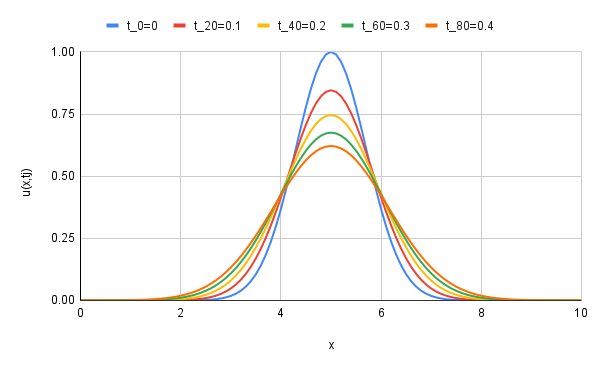
\includegraphics[width=0.85\textwidth]{rys/2.png}
\end{figure}

dla równania Burgersa
\begin{equation}
\begin{split}
& \frac{1}{k}(u_{i,j+1}-u_{i,j})+\frac{1}{4h}(u_{i+1,j}^{2}-u_{i-1,j}^{2})-\frac{\beta}{h^{2}}(u_{i+1,j}-2u_{i,j}+u_{i-1,j})=0\\
& u_{i,j+1}=u_{i,j}-\frac{k}{4h}(u_{i+1,j}^{2}-u_{i-1,j}^{2})+\frac{\beta k}{h^{2}}(u_{i+1,j}-2u_{i,j}+u_{i-1,j})
\end{split}
\end{equation}
\begin{figure}[h]
\caption{Równanie Burgersa, metoda Eulera}
\centering
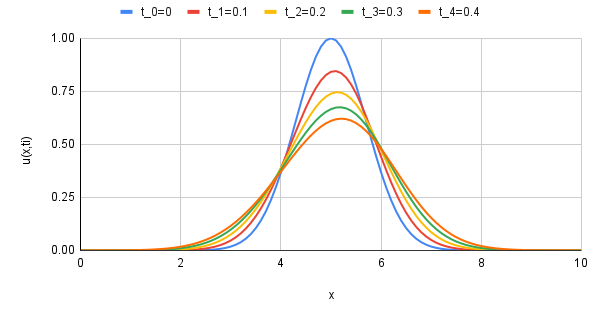
\includegraphics[width=0.85\textwidth]{rys/3.png}
\end{figure}
\newpage

Stosując metodę Rungego-Kutty drugiego rzędu:\\
dla równania transportu
\begin{equation}
\begin{split}
& v_{i,j+1}=u_{i,j}-\frac{k}{4h}(u_{i+1,j}-u_{i-1,j})\\
& u_{i,j+1}=u_{i,j}-\frac{k}{2h}(v_{i+1,j+1}-v_{i-1,j+1})
\end{split}
\end{equation}
\begin{figure}[h]
\caption{Równanie transportu, metoda RK2}
\centering
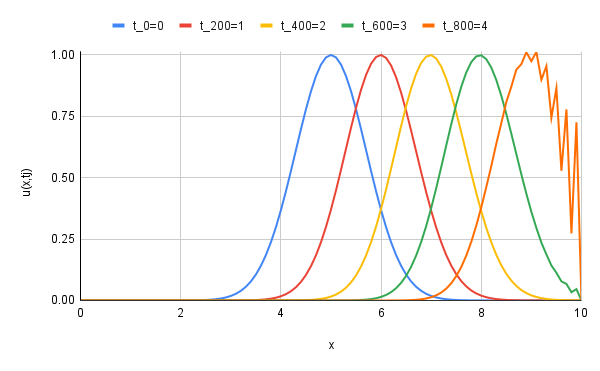
\includegraphics[width=0.85\textwidth]{rys/4.png}
\end{figure}

dla nielepkiego równania Burgersa
\begin{equation}
\begin{split}
& v_{i,j+1}=u_{i,j}-\frac{k}{8h}(u_{i+1,j}^{2}-u_{i-1,j}^{2})\\
& u_{i,j+1}=u_{i,j}-\frac{k}{4h}(v_{i+1,j+1}^{2}-v_{i-1,j+1}^{2})
\end{split}
\end{equation}
\begin{figure}[h]
\caption{Nielepkie równanie Burgersa, metoda RK2}
\centering
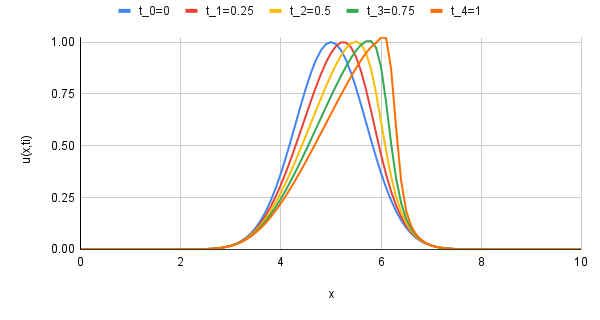
\includegraphics[width=0.85\textwidth]{rys/5.png}
\end{figure}
\newpage
\newpage

dla równania ciepła
\begin{equation}
\begin{split}
& v_{i,j+1}=u_{i,j}+\frac{\beta k}{2h^{2}}(u_{i+1,j}-2u_{i,j}+u_{i-1,j})\\
& u_{i,j+1}=u_{i,j}+\frac{\beta k}{h^{2}}(v_{i+1,j+1}-2v_{i,j+1}+v_{i-1,j+1})
\end{split}
\end{equation}
\begin{figure}[h]
\caption{Równanie ciepła, metoda RK2}
\centering
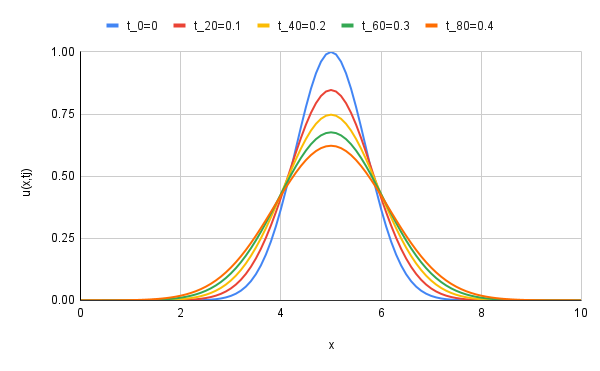
\includegraphics[width=0.85\textwidth]{rys/6.png}
\end{figure}

dla równania Burgersa
\begin{equation}
\begin{split}
& v_{i,j+1}=u_{i,j}-\frac{k}{8h}(u_{i+1,j}^{2}-u_{i-1,j}^{2})+\frac{\beta k}{2h^{2}}(u_{i+1,j}-2u_{i,j}+u_{i-1,j})\\
& u_{i,j+1}=u_{i,j}-\frac{k}{4h}(v_{i+1,j+1}^{2}-v_{i-1,j+1}^{2})+\frac{\beta k}{h^{2}}(v_{i+1,j+1}-2v_{i,j+1}+v_{i-1,j+1})
\end{split}
\end{equation}
\begin{figure}[h]
\caption{Równanie Burgersa, metoda RK2}
\centering
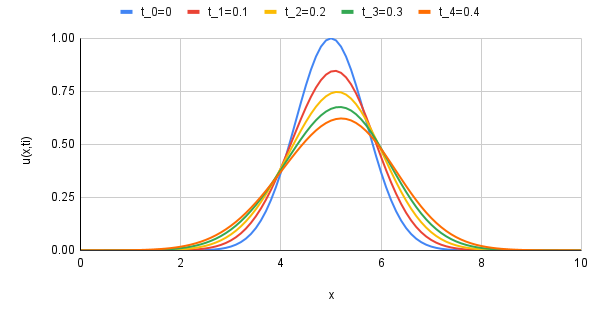
\includegraphics[width=0.85\textwidth]{rys/7.png}
\end{figure}
\newpage

Stosując metodę niejawną:\\
dla równania ciepła
\begin{equation}
\begin{split}
& \frac{1}{k}(u_{i,j}-u_{i,j-1})-\frac{\beta}{h^{2}}(u_{i+1,j}-2u_{i,j}+u_{i-1,j})=0\\
& u_{i,j-1}=-\frac{\beta k}{h^{2}}u_{i-1,j}+(1+2\frac{\beta k}{h^{2}})u_{i,j}-\frac{\beta k}{h^{2}}u_{i+1,j}
\end{split}
\end{equation}
\begin{center}
$A=
\begin{bmatrix}
1+2s & -s & 0 & \cdots & 0\\
-s & 1+2s & -s & \cdots & 0\\
0 & -s & 1+2s & \cdots & 0\\
\cdots & \cdots & \cdots & \cdots & \cdots\\
0 & 0 & 0 & \cdots & 1+2s\\
\end{bmatrix}$
$, s=\frac{\beta k}{h^{2}}$
\end{center}
\begin{equation}
u_{i,j}=A^{-1}u_{i,j-1}
\end{equation}
\begin{figure}[h]
\caption{Równanie ciepła, metoda niejawna}
\centering
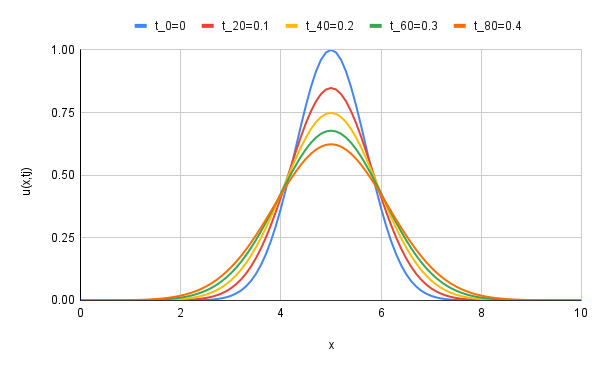
\includegraphics[width=0.85\textwidth]{rys/8.png}
\end{figure}
\newpage

dla równania Burgersa
\begin{equation}
\begin{split}
& \frac{1}{k}(u_{i,j}-u_{i,j-1})+\frac{1}{4h}(u_{i+1,j-1}^{2}-u_{i-1,j-1}^{2})-\frac{\beta}{h^{2}}(u_{i+1,j}-2u_{i,j}+u_{i-1,j})=0\\
& u_{i,j-1}-\frac{k}{4h}(u_{i+1,j-1}^{2}-u_{i-1,j-1}^{2})=-\frac{\beta k}{h^{2}}u_{i-1,j}+(1+2\frac{\beta k}{h^{2}})u_{i,j}-\frac{\beta k}{h^{2}}u_{i+1,j}
\end{split}
\end{equation}
\begin{center}
$A=
\begin{bmatrix}
1+2s & -s & 0 & \cdots & 0\\
-s & 1+2s & -s & \cdots & 0\\
0 & -s & 1+2s & \cdots & 0\\
\cdots & \cdots & \cdots & \cdots & \cdots\\
0 & 0 & 0 & \cdots & 1+2s\\
\end{bmatrix}$
$,s=\frac{\beta k}{h^{2}}$
\end{center}
\begin{equation}
u_{i,j}=A^{-1}(u_{i,j-1}-\frac{k}{4h}(u_{i+1,j-1}^{2}-u_{i-1,j-1}^{2}))
\end{equation}
\begin{figure}[h]
\caption{Równanie Burgersa, metoda niejawna}
\centering
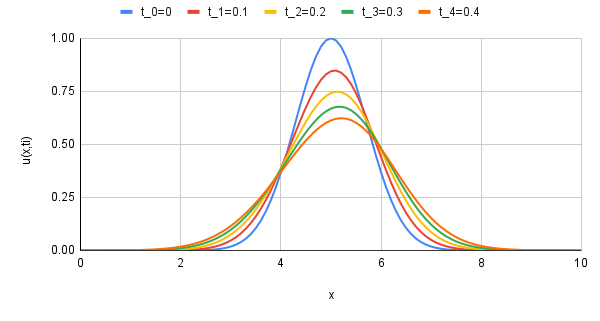
\includegraphics[width=0.85\textwidth]{rys/9.png}
\end{figure}
\newline
Algorytm, który realizuje opisaną metodę niejawną korzysta z procedury tri rozwiązującej układ równań o macierzy trójprzekątniowej. Metoda tri korzysta ze szczególnego przypadku eliminacji Gaussa w czasie $O(n)$, zamiast czasu $O(n^3)$ dla normalnego przypadku, co ogromnie przyspiesza znajdowanie rozwiązań.
\newpage

Uzyskaliśmy prawie identyczne wyniki za pomocą użycia metody Eulera, RK2 i niejawnej. Nie mogliśmy skorzystać z metody niejawnej dla równania transportu, ani dla nielepkiego równania Burgersa, ponieważ wymaga ona użycia macierzy kwadratowej (M=N), a dla tych równań ta równość nie zachodziła.\\

Dla równania transportu oraz nielepkiego równania Burgersa, jeśli $t$ przekroczy odpowiednią wartość, to przybliżone wartości $u$ zaczynają bardzo mocno odbiegać od rzeczywistych (dla równania transportu $t>3$, dla nielepkiego równania Burgersa, $t>1$).\\

Dla równania transportu, kolejne przesunięcia w czasie powodują uzyskanie maksymalnej wartości $u$ w kolejnych przesunięciach w przestrzeni.  Funkcja Gaussa zostaje jedynie przesunięta w prawo.  Zobrazowna zostaje liniowość.\\

Dla nielepkiego równania Burgera, kolejne przesunięcia w czasie powodują uzyskanie maksymalnej wartości $u$ w kolejnych przesunięciach w przestrzeni. Funkcja Gaussa nie zostaje jedynie przesunięta w prawo, tylko wolniej rośnie przed osiągnieciem kresu i szybciej opada po osiągnięciu kresu. Zobrazowna zostaje nieliniowość.\\

Dla równania ciepła, kolejne przesunięcia w czasie powodują zmniejszenie kresu funkcji Gaussa. Maksymalna wartość $u$ maleje w tym samym punkcie w przestrzeni (5) dla kolejnych czasów.\\ 

Dla równania Burgersa, kolejne przesunięcia w czasie powodują zmniejszenie kresu funkcji Gaussa oraz powodują przesunięcie w prawo. Maksymalna wartość $u$ maleje i przesuwa się w przestrzeni dla kolejnych czasów.\\

Zwiększanie współczynnika $\beta$ powoduje zmniejszenie kresu $u(x,t)$. Dzieje się tak do około $\beta$ = 1.2, po czym rozwiązanie staje się całkowicie niepoprawne.\\
\begin{figure}[h]
\caption{Równanie Burgersa, metoda Eulera, $\beta$=1.3}
\centering
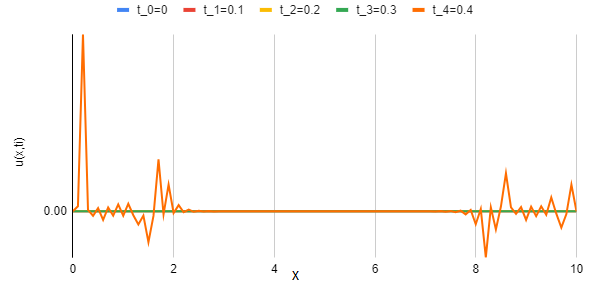
\includegraphics[width=0.85\textwidth]{rys/10.png}
\end{figure}

Program komputerowy w języku C++ wyznaczający powyższe rozwiązania został dołączony w Dodatku A.

\documentclass[a4paper,11pt]{article}
\usepackage[T1]{fontenc}
\usepackage[utf8]{inputenc}
\usepackage{xcolor}
\usepackage{geometry}
\usepackage{subfig}
\geometry{left=2.5cm,right=2.5cm,top=2.5cm,bottom=2.5cm}
\usepackage{multicol}
\usepackage{fancyhdr}
\linespread{1.5}
\colorlet{shadecolor}{gray!40}
\usepackage{listings}
\usepackage{subcaption}
\usepackage{pdfpages}
\lstdefinestyle{mystyle}{
	%backgroundcolor=\color{shadecolor}
	commentstyle=\footnotesize\color{blue},
	keywordstyle=\color{red},
	numberstyle=\footnotesize\color{black},
	stringstyle=\color{black},
	basicstyle=\footnotesize,
	breakatwhitespace=false,
	breaklines=true, captionpos=b,
	keepspaces=true, numbers=left,
	numbersep=5pt, showspaces=false,
	showstringspaces=false, showtabs=false,
	tabsize=2,	
}
\lstset{style=mystyle}
\setlength{\parindent}{1.25cm}


\usepackage{amsmath}
\usepackage{graphicx}
\usepackage{hyperref}
\usepackage{fancyhdr}
\usepackage{tocloft}

\begin{document}

	\section{Opis programu transformaty Hopf Cole'a}
Program komputerowy został napisany na podstawie wzorów~\ref{14a}:
\begin{equation}
\label{14a}
\begin{split}
    \theta_{i,j+1}=(1-2r)\theta_{i,j}+2r\theta_{i+1,j}, \ \ i=0\\
    \theta_{i,j+1}=2r\theta_{i-1,j}+(1-2r)\theta_{i,j}+r\theta_{i+1,j}, \ \ 1\le i\le N-1\\
    \theta_{i,j+1}=2r\theta_{i-1,j}+(1-2r)\theta_{i,j}
\end{split}
\end{equation}.
Natomiast równanie na u zostało zrobione z wzoru:
\begin{equation}
    u(x_i,t_j)=-\frac{\beta}{h}\left(\frac{\theta_{i+1,j}-\theta_{i-1,j}}{\theta_{i,j}}\right)\ \ 1\le i\le N-1
\end{equation}.
Gdzie $\beta$ jest współczynnikiem lepkości, h krokiem przestrzennym, a k - krokiem czasowym.
	\subsection{transformataHopfCole.h}
	Plik nagłówkowy zawiera definicje metod klasy transformaty. Na początku zostały dołączone wszystkie klasy, które są potrzebne do działania programu, jak pokazuje listing~\ref{poczatekPlikuH}.
		\begin{lstlisting}[caption={początek pliku transformataHopfCole.h},label={poczatekPlikuH}, language=C++]]
		#pragma once
		#include <vector>
		#include <cmath>
		#include <algorithm>
		#include <conio.h>
		#include <math.h>;\end{lstlisting}
	Następnie zostały napisana dyrektywa, która pozwala na używanie wszystkich nazw z~przestrzeni nazw "std" bez konieczności ich niefiksowania. Przestrzeń nazw definiuję standardowych klas i~funkcji z~biblioteki standardowej w~C++, takich jak "cout", "vecotr", "string", co skraca trochę kod. Potem zostały definiowanie stała Pi oraz~e, jeśli nie są szybciej zdefiniowanie, co przedstawia listing~\ref{definiowanieStałych}. 
	\begin{lstlisting}[caption={początek pliku definiowanieStałych},label={zdefiniowanie stałych}, language=C++]]
		using namespace std;
		#ifndef M_PI
		#define M_PI 3.14159265358979323846
		#endif
		
		#ifndef M_E
		#define M_E 2.71828182845904523536
		#endif\end{lstlisting}
		
	Potem została zdefiniowania klasa, w~której są wszystkie metody oraz stale potrzebnie do pracy programu.
			\begin{lstlisting}[caption={klasa tranformataHopfCofe},label={klasa}, language=C++]
			class transformataHopfCole {
				const double k = 0.005, h = 0.1;
                const int N = 1 / h + 1;      // liczba punktów siatki
				const double n = ((0.5 * pow(h, 2)) / k) - 0.01;
				const double r = n*k / pow(h, 2);
				double t = 0;
				
				vector<double>theta;
				vector<double>mu;
				vector<double> inicjacja_u(); //wzror 4 z pracy
				vector<double>inicjacjaThetaX0(); //wzor 8 z pracy
				vector<double>liczenieThetaOdCzasu();
				
				vector<double>liczenieMu(vector<double>newMu);//wzor 15
				void zapisDoPliku(vector<double> Theta, double newT);
				public:
				void wynikiKonczowe();
			};\end{lstlisting}
		Pierwsza stała oznacza liczbę punktów, "k" odpowiada za krok czasowy, natomiast "h" za krok przestrzennego w~dyskretyzacji przestrzennej.\\
		W~8~i~9~linii zostały inicjowanie vectoru, gdzie zostaniom zapisanie wyniki programu. W~kolejnych trzech linach zostały już zdefiniowanie klasy, które krok po kroku będą obliczały wynik końcowy oraz w linii~14.\\
		Przedostatnia prywatna metoda służy, by otrzymanie wyniki zostały zapisanie do pliku. Ostaną metodą jest "wynikiKoncowe()", która jest publiczna. 
		\subsection{transformataHopfCole.cpp}
		W kolejnym pliku znajdują się ciała metod klasy. Na początku pliku zostały załączone biblioteki oraz własna klasa do prawidłowego działania programu. 
					\begin{lstlisting}[caption={poczadek pliku transformataHopfCole.cpp},label={poczadek.cpp}, language=C++]
#include "transformataHopfCole.h"
#include <iostream>
#include <fstream>
#include <string>\end{lstlisting}
	\	Następne jest ciało metody inicjacjaThetaX0 co przedstawia listing~\ref{inicjacjaThetaX0}. Ta metoda ma na celu inicjacji~$\theta$ dla czasu zerowego. Pętla służy do wygenerowana dla wszystkich~$\theta$ wartości początkowych, z~których potem zostaną wykorzystanie do dalszych obliczeń. Pod koniec metody zostanie wywołania kolejna metoda, która zapiszę wartości do pliku tekstowego oraz zwrócenie tych wartości do vectora.
						\begin{lstlisting}[caption={ciało metody inicjacjaThetaX0},label={inicjacjaThetaX0}, language=C++]
		vector<double> transformataHopfCole::inicjacjaThetaX0() {
			vector<double>newTheta;
			for (int i = 0; i < N; ++i) {
				double potega = (-1 / (2 * M_PI * n)) * (1 - cos(M_PI * (i * h)));
				newTheta.push_back(exp(potega));
			}
			zapisDoPliku(liczenieMu(newTheta), 0);
			return newTheta;
			}\end{lstlisting}
		Kolejną metodą jest "liczenieThetaOdCzasu" (listing~\ref{liczenieThetaOdCzasu}). Metoda ma na celu policzenie~$\theta$ dla czasu. Pierwsza pętla służy do policzenie~"t", czyli kroku czasowego. Potem jest zdefiniowany nowy vector, w którym zostaną zapisanie nowe wartości. Druga pętla służy do policzenia dla $\theta$ od~1 do~N-1. Po drugiej pętli zostaną nadpisanie wartości dla theyaDlaCzasu nowymi wartościami dla konkretnego czasu. Na końcu jest wywołania metoda, która otrzymanie wyniki zapiszę do pliku. Na samym końcu zostanie zwrócony vector.   
								\begin{lstlisting}[caption={ciało metody liczenieThetaOdCzasu},label={liczenieThetaOdCzasu}, language=C++]
vector<double> transformataHopfCole::liczenieThetaOdCzasu() {
	vector<double>thetaDlaCzasu(N);
	thetaDlaCzasu = theta;
	for (int j = 1; j < 3000; ++j) {
		t = j * k;
		vector<double>v(N);
		v[0] = (1 - 2 * r) * thetaDlaCzasu[0] + 2 * r * thetaDlaCzasu[1]; //warunki brzegowe  
		v[N - 1] = 2 * r * thetaDlaCzasu[N - 2] + (1 - 2 * r) * thetaDlaCzasu[N - 1];
		for (int i = 1; i < (N - 1); ++i) {
			double wynik = r * thetaDlaCzasu[i - 1] + (1 - 2 * r) * thetaDlaCzasu[i] + r * thetaDlaCzasu[i + 1];
			v[i] = wynik;
		}
		thetaDlaCzasu = v;
		zapisDoPliku(liczenieMu(thetaDlaCzasu), t);
		
	}
	return thetaDlaCzasu;
	}\end{lstlisting}
Kolejną metodą jest "liczenieMu", która wykorzystuję $\theta$ od czasu do policzenia $u(x,t)$. Na wyraz 0 i~(N-1) jest przypisana wartość~0, co wynika z warunki początkowego i~końcowego. Kolejne wartości są liczone w pętli for, jak pokazuje listing~\ref{liczenieMu}. 
\begin{lstlisting}[caption={ciało metody liczenieMu},label={liczenieMu}, language=C++]
vector<double> transformataHopfCole::liczenieMu(vector<double> newMu) {
	vector<double>newMu1(N);
	newMu1[0] = 0;//warunek poczatkowy
	newMu1[N - 1] = 0;//warunek koncowy
	for (int i = 1; i < (N - 1); ++i) {
		newMu1[i] = (-(n / h) * ((newMu[i + 1] - newMu[i - 1]) / newMu[i]));
	}
	
	return newMu1;
	}\end{lstlisting}
Przedostatnią metodą jest "zapisDoPliku", który ma na celu otrzymanych wyników zapisach do pliku. Na początku jest inicjowany string, który będzie nazwą pliku. Potem program tworzy nowy plik, jeśli nie istnieje, jak istnieje to zawartość zostanie zastąpiona. Potem w warunku jest sprawdzenie czy udało się otworzyć plik, jeśli nie to pojawi się odpowiednia informacja. Pętla for ma na celu zapisanie wszystkich punktów do pliku. Na końcu program zamyka plik, gdy już skończył pracę.
\begin{lstlisting}[caption={metoda zapisDoPliku},label={ZapisDoPliku}, language=C++]
void transformataHopfCole::zapisDoPliku(vector<double> newMu, double newT) {
	string nazwaPliku = "Wyniki1DlaT" + to_string(newT) + ".txt";
	std::ofstream plik(nazwaPliku);
	
	// Sprawdzamy, czy plik został otwarty poprawnie
	if (!plik) {
		std::cerr << "Nie można otworzyć pliku!" << std::endl;
		return;
	}
	for (int i = 0; i < size(newMu); ++i) {
		
		plik << (i * h) << " " << newMu[i] << '\n';
	}
	
	// Zamykamy plik
	plik.close();
}\end{lstlisting}
Ostaną metodą są "wynikiKoncowe", który na początku wywołuje metodę "inicjacjaThetaX0", następnie "liczenieThetaOdCzasu". Kolejne metody nie są potrzebne by je wywołać, z powodu, że metoda "liczenieThetaOdCzasu" wywołuje metodę która liczy $u(x,t)$ i metodą, która zapisuję dane do pliku. 
\begin{lstlisting}[caption={metoda wynikiKonczowe},label={wynikiKonczowe}, language=C++]
void transformataHopfCole::wynikiKonczowe() {
	theta = inicjacjaThetaX0();
	theta = liczenieThetaOdCzasu();
	}\end{lstlisting}
\subsection{transformata.cpp}
Kolejnym plikiem jest transformata.cpp, który ma funkcję główną main.cpp. Która na początku ma dołączona klasę. Następnie w main tworzy się obiekt klasy transformataHopfCole, a następnie wywołuję się metodę klasy, by program policzył nam wyniki. 
\begin{lstlisting}[caption={transformata.cpp},label={transformata}, language=C++]
#include "transformataHopfCole.h"
int main()
{
	transformataHopfCole Burger;
	Burger.wynikiKonczowe();
}
\end{lstlisting}
\section{wyniki}
Wygenerowano wykresy dla $k=0.0005$ i~$h=0.1$. Dla coraz większego czasu można zauważyć, że amplituda rozwiązana maleje, można to zauważyć na rys~\ref{fig:wykresy-dla-uxt}, wyniki punktów wykresu są przedstawione na tabelkach~\ref{tab1} i~\ref{tab2}.\\
\begin{figure}
	\centering
	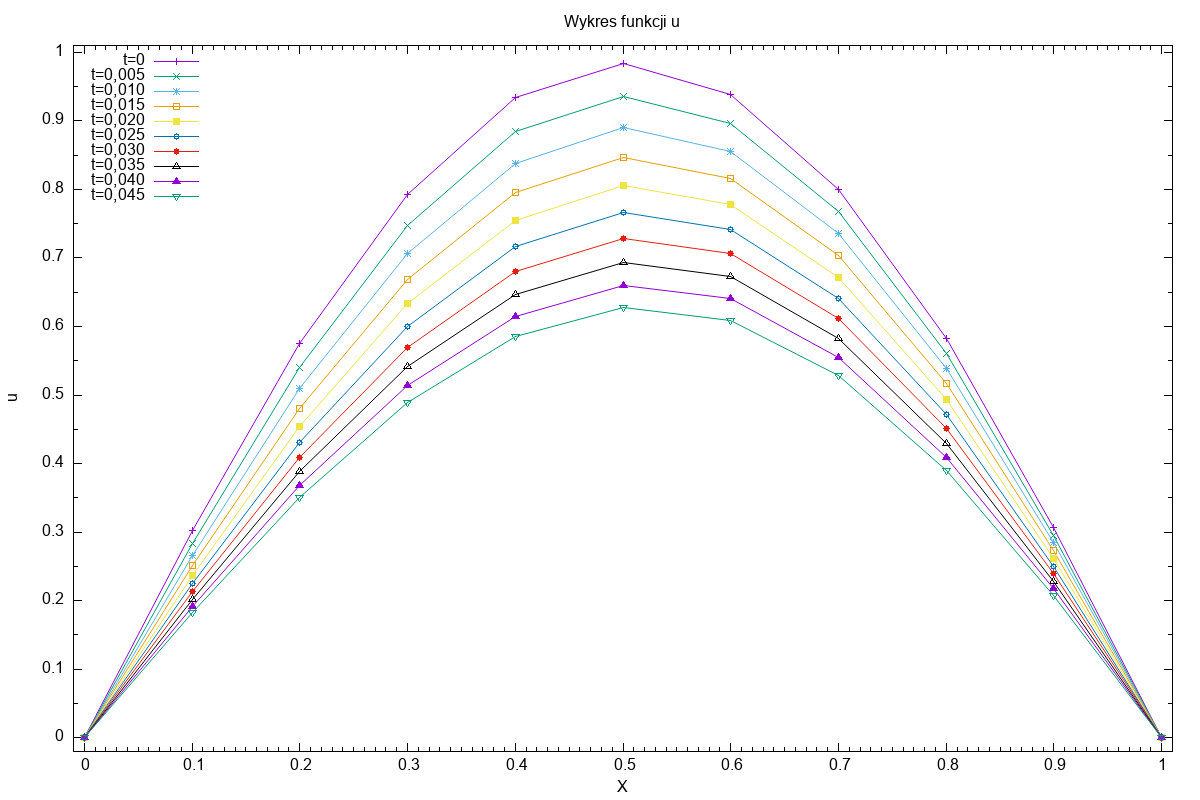
\includegraphics[width=0.7\linewidth]{rys/wykresy dla u(x,t).png}
	\caption{k = 0.005, h = 0.1}
	\label{fig:wykresy-dla-uxt}
\end{figure}
\begin{table}[]
	\begin{tabular}{|l|l|l|l|l|l|l|}
		\hline
x\textbackslash{}t & 0        & 0.005    & 0,010    & 0.015    & 0.020    & 0.025    \\ \hline
0                  & 0        & 0        & 0        & 0        & 0        & 0        \\ \hline
0.1                & 0.301705 & 0.283068 & 0.266381 & 0.251276 & 0.237487 & 0.224811 \\ \hline
0.2                & 0.574577 & 0.540199 & 0.509139 & 0.480833 & 0.454852 & 0.430863 \\ \hline
0.3                & 0.792316 & 0.747317 & 0.706078 & 0.668073 & 0.632879 & 0.600146 \\ \hline
0.4                & 0.933565 & 0.88415  & 0.838007 & 0.794843 & 0.754384 & 0.716382 \\ \hline
0.5                & 0.984036 & 0.93621  & 0.890555 & 0.847073 & 0.805711 & 0.766389 \\ \hline
0.6                & 0.938116 & 0.896627 & 0.856073 & 0.816677 & 0.778584 & 0.741879 \\ \hline
0.7                & 0.799679 & 0.767504 & 0.735313 & 0.703418 & 0.672066 & 0.641447 \\ \hline
0.8                & 0.581939 & 0.560385 & 0.53838  & 0.516199 & 0.494079 & 0.472219 \\ \hline
0.9                & 0.306254 & 0.295543 & 0.284455 & 0.273144 & 0.26175  & 0.250398 \\ \hline
1                  & 0        & 0        & 0        & 0        & 0        & 0        \\ \hline\end{tabular}
	\caption{Wyniki dla k=0.005,h=0.1, dla czasu od 0 do 0.025}
	\label{tab1}
\end{table}
\begin{table}[]
	\begin{tabular}{|l|l|l|l|l|l|}
		\hline
		x\textbackslash{}t & 0.030    & 0.35     & 0.40     & 0.45     & 0.45     \\ \hline
		0                  & 0        & 0        & 0        & 0        & 0        \\ \hline
		0.1                & 0.213091 & 0.202201 & 0.192041 & 0.182528 & 0.182528 \\ \hline
		0.2                & 0.408602 & 0.387857 & 0.368453 & 0.350247 & 0.350247 \\ \hline
		0.3                & 0.569591 & 0.540975 & 0.514101 & 0.488803 & 0.488803 \\ \hline
		0.4                & 0.680618 & 0.6469   & 0.615061 & 0.584955 & 0.584955 \\ \hline
		0.5                & 0.729015 & 0.693493 & 0.659731 & 0.627636 & 0.627636 \\ \hline
		0.6                & 0.706609 & 0.672786 & 0.640407 & 0.609451 & 0.609451 \\ \hline
		0.7                & 0.611699 & 0.582919 & 0.555172 & 0.528496 & 0.528496 \\ \hline
		0.8                & 0.450776 & 0.429873 & 0.409598 & 0.390013 & 0.390013 \\ \hline
		0.9                & 0.239189 & 0.228205 & 0.217507 & 0.207141 & 0.207141 \\ \hline
		1                  & 0        & 0        & 0        & 0        & 0        \\ \hline
	\end{tabular}
		\caption{Wyniki dla k=0.005,h=0.1, dla czasu od 0.030 do 0.045}
	\label{tab2}
\end{table}
Można zauważyć, że jak zmniejszymy k do 0.0005, to można zauważyć, że dla czasu 0 funkcja jest trójkąta. Natomiast dla większego czasu można zauważyć, że funkcja się powoli zaokrągla i~przypomina coraz bardziej wykres dla sinusa, można to zauważyć na rys~\ref{wyk2}. \\
Na pozostały wykresach~\ref{wyk11,wyk12,wyk13}, można zauważyć jak zmiana współczynników wpływa na generowanie wykresów. Jak zmienia się współczynnik lepkości to można zauważyć że amplituda zwiększa się lub zamieszcza, zależy od wartości. Natomiast gdy się zmienia krok przestrzeni to zmienia się ilość punktów na osi~x, a gdy ostatnią wartość się zmieni (krok czasowy), to powstaje więcej lub mniej rozwiązań $\theta$ od czasu.Na każdych z wykresów można zauważyć, że dla coraz większego czasu amplituda zamieszcza się oraz lekko przesuwa się w prawą stronę.\\
Gdy warunek na stabilność, $k/h^2\le0.5$ jest nie zachowany to program wygeneruję wyniki, ale w pliku tekstowym pojawiają się wartości "ind", których nie można przeanalizować oraz naszkicować na wykresie tych punktów.\\
\begin{figure}[ht]
    \centering
    \subfloat[$\beta$=0.1, k=0.001, h=0.025]{%
        \includegraphics[width=0.3\linewidth]{rys/wykresy dla u(x,t) v=0,1 k = 0.001, h = 0.025.png}
        \label{wyk11}
    }
    \hfill
    \subfloat[$\beta$=0.1, k=0.005, h=0.1]{%
        \includegraphics[width=0.3\linewidth]{rys/wykresy dla u(x,t) v=0,1 k = 0.005, h = 0.1.png}
        \label{wyk12}
    }
    \hfill
    \subfloat[$\beta$=0.99, k=0.005, h=0.1]{%
        \includegraphics[width=0.3\linewidth]{rys/wykresy dla u(x,t) v=0,99 k = 0.005, h = 0.1.png}
        \label{wyk13}
    }
    \caption{Wykresy dla rozwiązań transformaty}
    \label{Wykresy dla rożwiązań}
\end{figure}
Przedstawione na wykresach~\ref{fig:wykresy_dla_rozwiazan}, można zobaczyć, że dla większego czasu, że wykres coraz mniej przypomina wykres sinusa. Może wynikać to z błędach numerycznych, które z każdym rozwiązaniem gromadzą się i robią się coraz większe. 
\begin{figure}[]
    \centering
    \subfloat[$\beta=12000$, $k=0.00001$, $h=0.01$]{%
        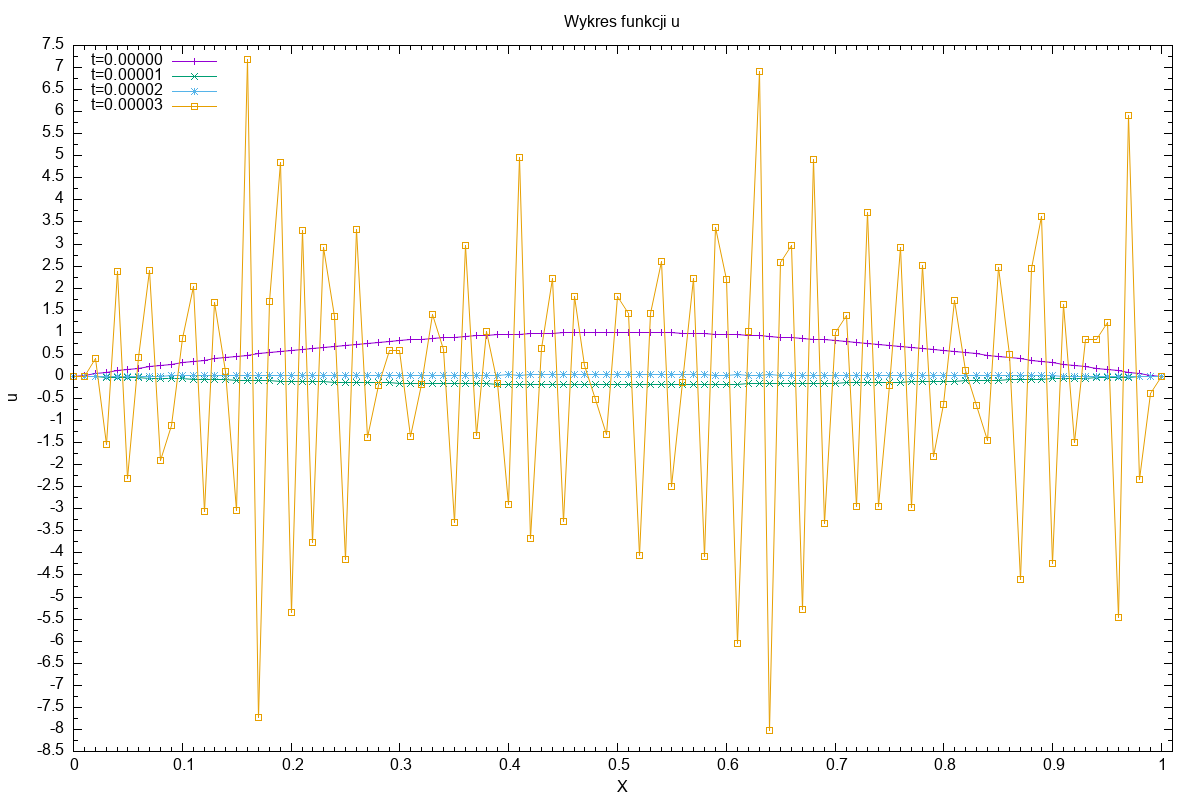
\includegraphics[width=0.45\linewidth]{rys/zl.png}
        \label{wyk21}
    }
    \hfill
    \subfloat[$\beta=12000$, $k=0.00001$, $h=0.1$]{%
        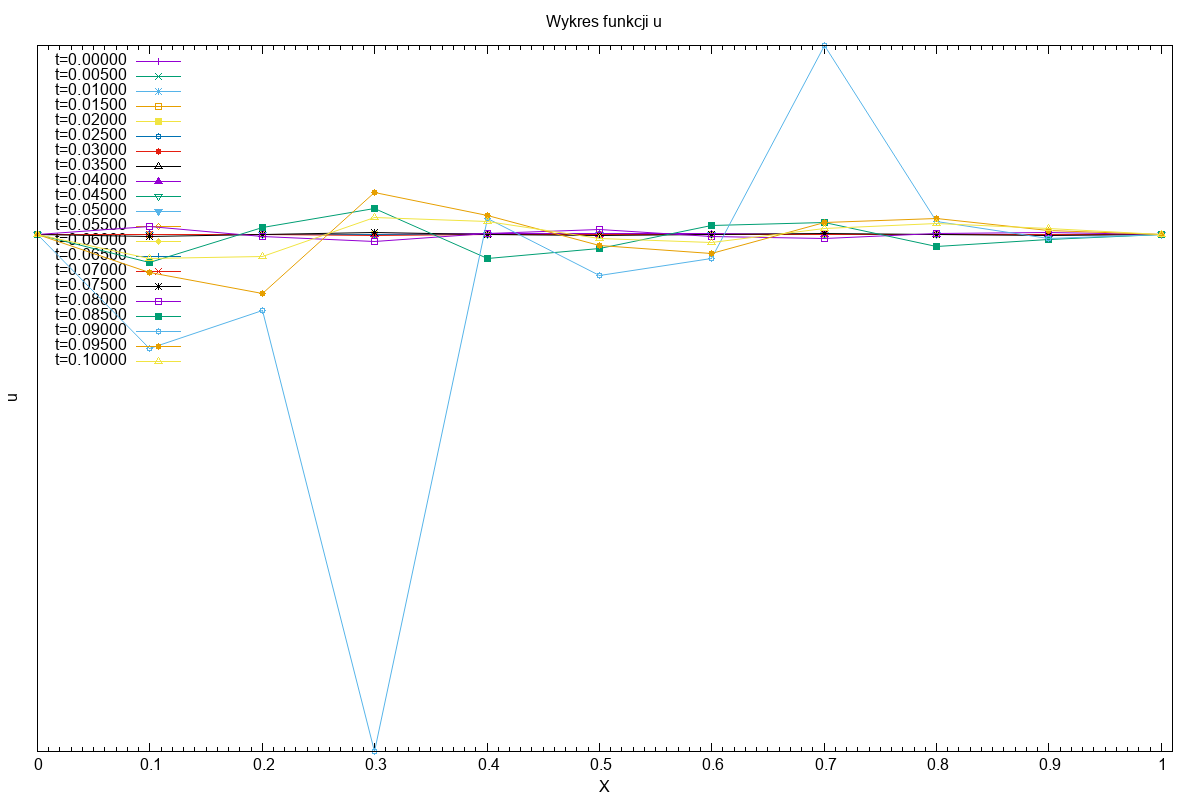
\includegraphics[width=0.45\linewidth]{rys/zl1.png}
        \label{wyk22}
    }
    \caption{Źle dobrane warunki}
    \label{fig:wykresy_dla_rozwiazan}
\end{figure}
\section{Podsumowanie}
W tej pracy przybliżyliśmy równanie Burgersa oraz jego zastosowania, transformację Hopf-Cole'a, rozwiązanie analityczne oraz metody numeryczne, w tym metodę różnic skończonych, metodę Eulera oraz metodę Rungego-Kutty.

\newpage
\section{dodatek A}
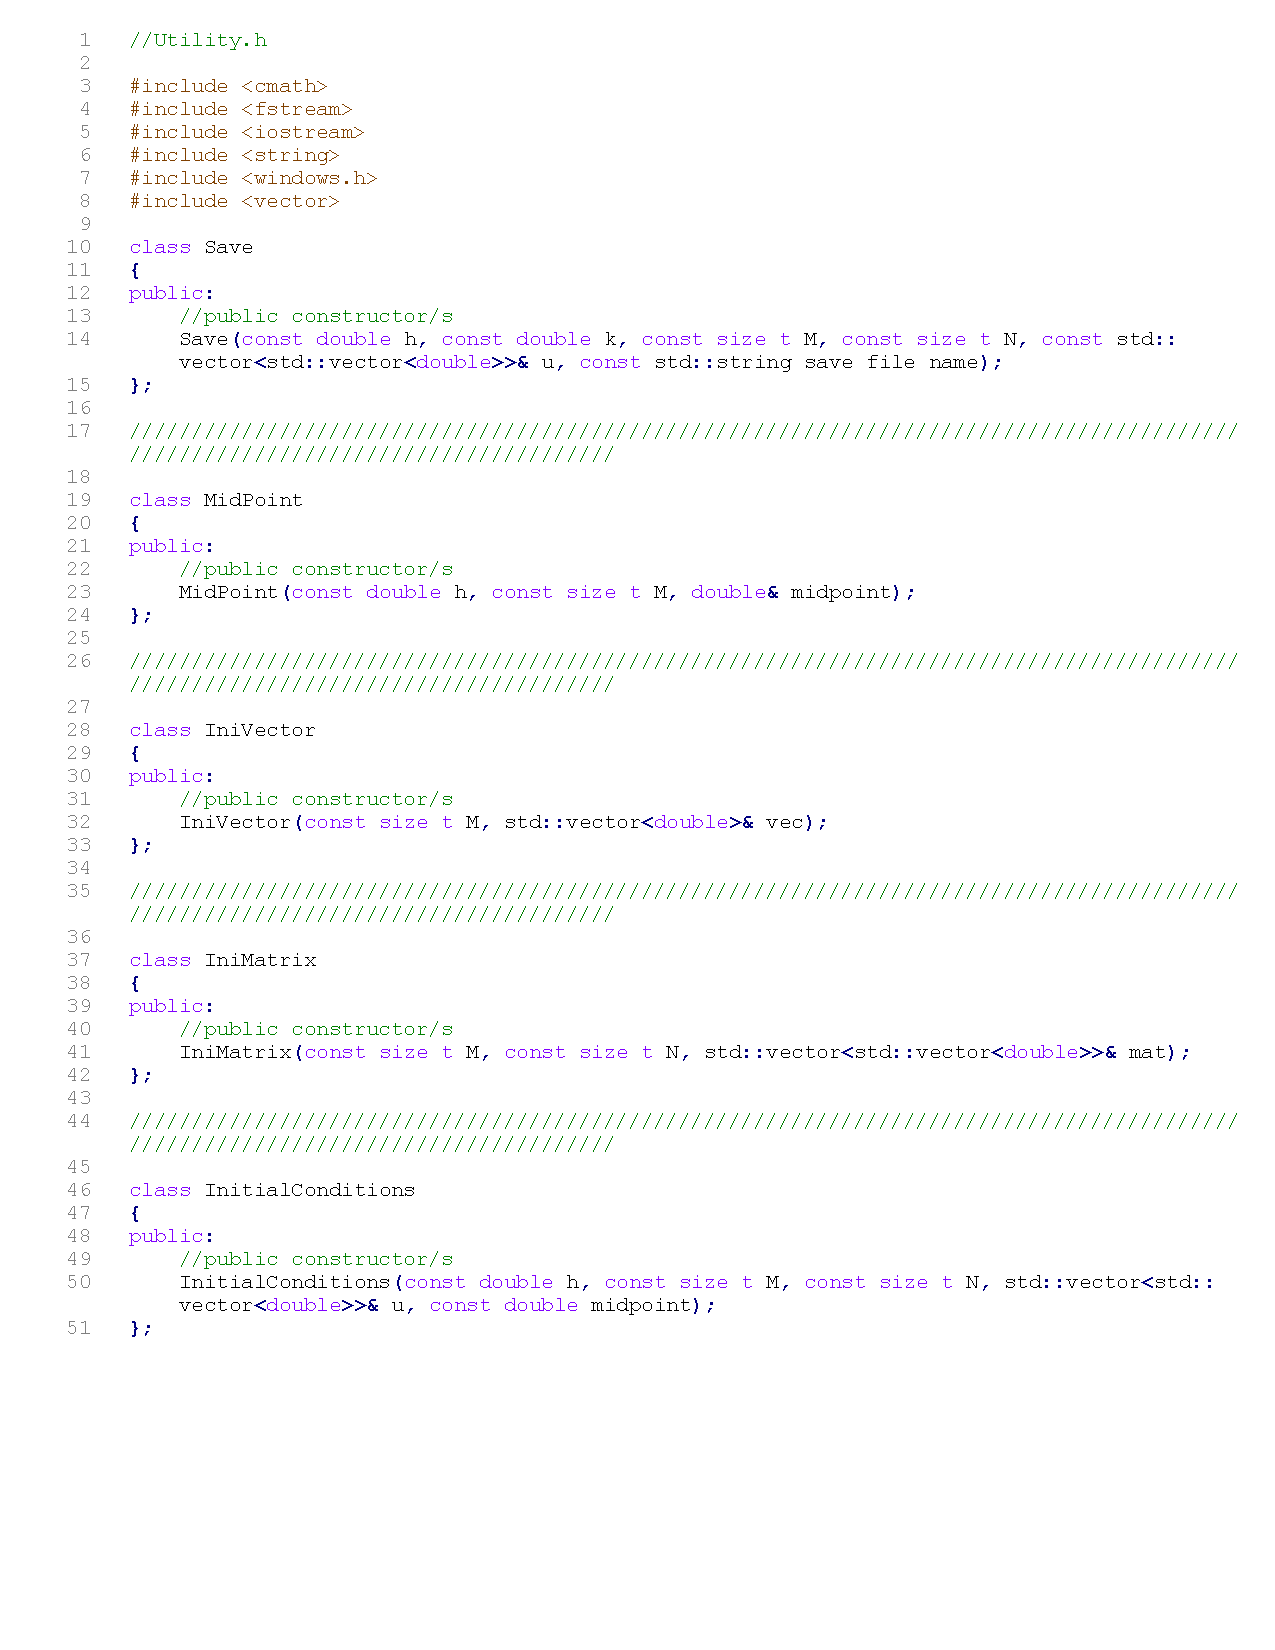
\includepdf[pages={1}]{rys/Dodatek_A.pdf}
\includepdf[pages={2}]{rys/Dodatek_A.pdf}
\includepdf[pages={3}]{rys/Dodatek_A.pdf}
\includepdf[pages={4}]{rys/Dodatek_A.pdf}
\includepdf[pages={5}]{rys/Dodatek_A.pdf}
\includepdf[pages={6}]{rys/Dodatek_A.pdf}
\includepdf[pages={7}]{rys/Dodatek_A.pdf}
\includepdf[pages={8}]{rys/Dodatek_A.pdf}
\includepdf[pages={9}]{rys/Dodatek_A.pdf}
\includepdf[pages={10}]{rys/Dodatek_A.pdf}
\includepdf[pages={11}]{rys/Dodatek_A.pdf}
\includepdf[pages={12}]{rys/Dodatek_A.pdf}
\includepdf[pages={13}]{rys/Dodatek_A.pdf}
\includepdf[pages={14}]{rys/Dodatek_A.pdf}
\includepdf[pages={15}]{rys/Dodatek_A.pdf}
\includepdf[pages={16}]{rys/Dodatek_A.pdf}
\includepdf[pages={17}]{rys/Dodatek_A.pdf}
\includepdf[pages={18}]{rys/Dodatek_A.pdf}
\includepdf[pages={19}]{rys/Dodatek_A.pdf}
\includepdf[pages={20}]{rys/Dodatek_A.pdf}
\includepdf[pages={21}]{rys/Dodatek_A.pdf}
\section{dodatek B}

\subsection{transformata.cpp}
\begin{lstlisting}[caption={transformata.cpp},label={transformataCalyKod}, language=C++]
	#include "transformataHopfCole.h"
	int main()
	{
		transformataHopfCole Burger;
		Burger.wynikiKonczowe();
	}
\end{lstlisting}
\subsection{transformataHopfCole.h}
\begin{lstlisting}[caption={transformataHopfCole.h},label={transformataHopfCole.hCalyKod}, language=C++]
#pragma once
#include <vector>
#include <cmath>
#include <algorithm>
#include <conio.h>
#include <math.h>
using namespace std;
#ifndef M_PI
#define M_PI 3.14159265358979323846
#endif

#ifndef M_E
#define M_E 2.71828182845904523536
#endif

class transformataHopfCole {
	
	const double k = 0.005, h = 0.1;
    const int N = 1 / h + 1; // liczba punktów siatki
	const double n = ((0.5 * pow(h, 2)) / k) - 0.01;
	const double r = n * k / pow(h, 2);
	double t = 0;
	
	vector<double>theta;
	vector<double>mu;
	vector<double>inicjacjaThetaX0(); //wzor 8 z pracy
	vector<double>liczenieThetaOdCzasu();
	
	vector<double>liczenieMu(vector<double>newMu);//wzor 15
	void zapisDoPliku(vector<double> Theta, double newT);
	public:
	void wynikiKonczowe();
	
};
\end{lstlisting}
\subsection{transformataHopfCole.cpp}
\begin{lstlisting}[caption={transformataHopfCole.cpp},label={transformataHopfColeCalyKod.cpp}, language=C++]
#include "transformataHopfCole.h"
#include <iostream>
#include <fstream>
#include <string>



vector<double> transformataHopfCole::inicjacjaThetaX0() {
	vector<double>newTheta;
	for (int i = 0; i < N; ++i) {
		double potega = (-1 / (2 * M_PI * n)) * (1 - cos(M_PI * (i * h)));
		newTheta.push_back(exp(potega));
	}
	zapisDoPliku(liczenieMu(newTheta), 0);
	return newTheta;
}

vector<double> transformataHopfCole::liczenieThetaOdCzasu() {
	vector<double>thetaDlaCzasu(N);
	thetaDlaCzasu = theta;
	for (int j = 1; j < 10; ++j) {
		t = j * k;
		vector<double>v(N);
		v[0] = (1 - 2 * r) * thetaDlaCzasu[0] + 2 * r * thetaDlaCzasu[1]; //warunki brzegowe  
		v[N - 1] = 2 * r * thetaDlaCzasu[N - 2] + (1 - 2 * r) * thetaDlaCzasu[N - 1];
		for (int i = 1; i < (N - 1); ++i) {
			double wynik = r * thetaDlaCzasu[i - 1] + (1 - 2 * r) * thetaDlaCzasu[i] + r * thetaDlaCzasu[i + 1];
			v[i] = wynik;
		}
		thetaDlaCzasu = v;
		zapisDoPliku(liczenieMu(thetaDlaCzasu), t);
		
	}
	return thetaDlaCzasu;
}

vector<double> transformataHopfCole::liczenieMu(vector<double> newMu) {
	vector<double>newMu1(N);
	newMu1[0] = 0;//warunek poczatkowy
	newMu1[N - 1] = 0;//warunek koncowy
	for (int i = 1; i < (N - 1); ++i) {
		newMu1[i] = (-(n / h) * ((newMu[i + 1] - newMu[i - 1]) / newMu[i]));
	}
	
	return newMu1;
}

void transformataHopfCole::zapisDoPliku(vector<double> newMu, double newT) {
	string nazwaPliku = "Wyniki1DlaT" + to_string(newT) + ".txt";
	std::ofstream plik(nazwaPliku);
	
	// Sprawdzamy, czy plik został otwarty poprawnie
	if (!plik) {
		std::cerr << "Nie można otworzyć pliku!" << std::endl;
		return;
	}
	for (int i = 0; i < size(newMu); ++i) {
		
		plik << (i * h) << " " << newMu[i] << '\n';
	}
	
	// Zamykamy plik
	plik.close();
}

void transformataHopfCole::wynikiKonczowe() {
	theta = inicjacjaThetaX0();
	theta = liczenieThetaOdCzasu();
}

\end{lstlisting}


\end{document}